\esSezione{Comunicazione con handshaking}\label{sec:esercizio8-1}

\begin{traccia}
Progettare, implementare in VHDL e testare mediante simulazione un sistema formato da due nodi, A e B, che comunicano con un protocollo di handshaking. Ciascun nodo dispone di una memoria interna con $N$ stringhe di $M$ bit, indicate rispettivamente con $X(i)$ e $Y(i)$, per $i = 0, \dots, N-1$. Il nodo A trasmette a B ogni stringa $X(i)$; B, ricevutala, calcola $S(i) = X(i) + Y(i)$ e memorizza la somma nella propria memoria. La somma può essere descritta in modo comportamentale, mentre in entrambi i nodi deve essere presente un componente contatore che scandisce le stringhe e determina la fine della comunicazione.
\end{traccia}

\progetto

Il sistema è composto da due entità, \texttt{system\_A} e \texttt{system\_B}, collegate dai segnali \texttt{req}, \texttt{ack} e \texttt{data}. Il nodo A contiene una Control Unit, una ROM con le stringhe $X(i)$ e un contatore che ne scandisce gli indirizzi. Il nodo B contiene una Control Unit, un registro che cattura il dato ricevuto, un adder, una memoria con le stringhe $Y(i)$ (nella quale viene scritta anche la somma) e un contatore degli indirizzi. I due nodi lavorano con clock indipendenti, quindi la sincronizzazione è affidata al solo handshaking. La figura~\ref{fig:esercizio8-1:architettura} illustra l'architettura complessiva, con il clock omesso per chiarezza.

\begin{figure}[H]
  \centering
  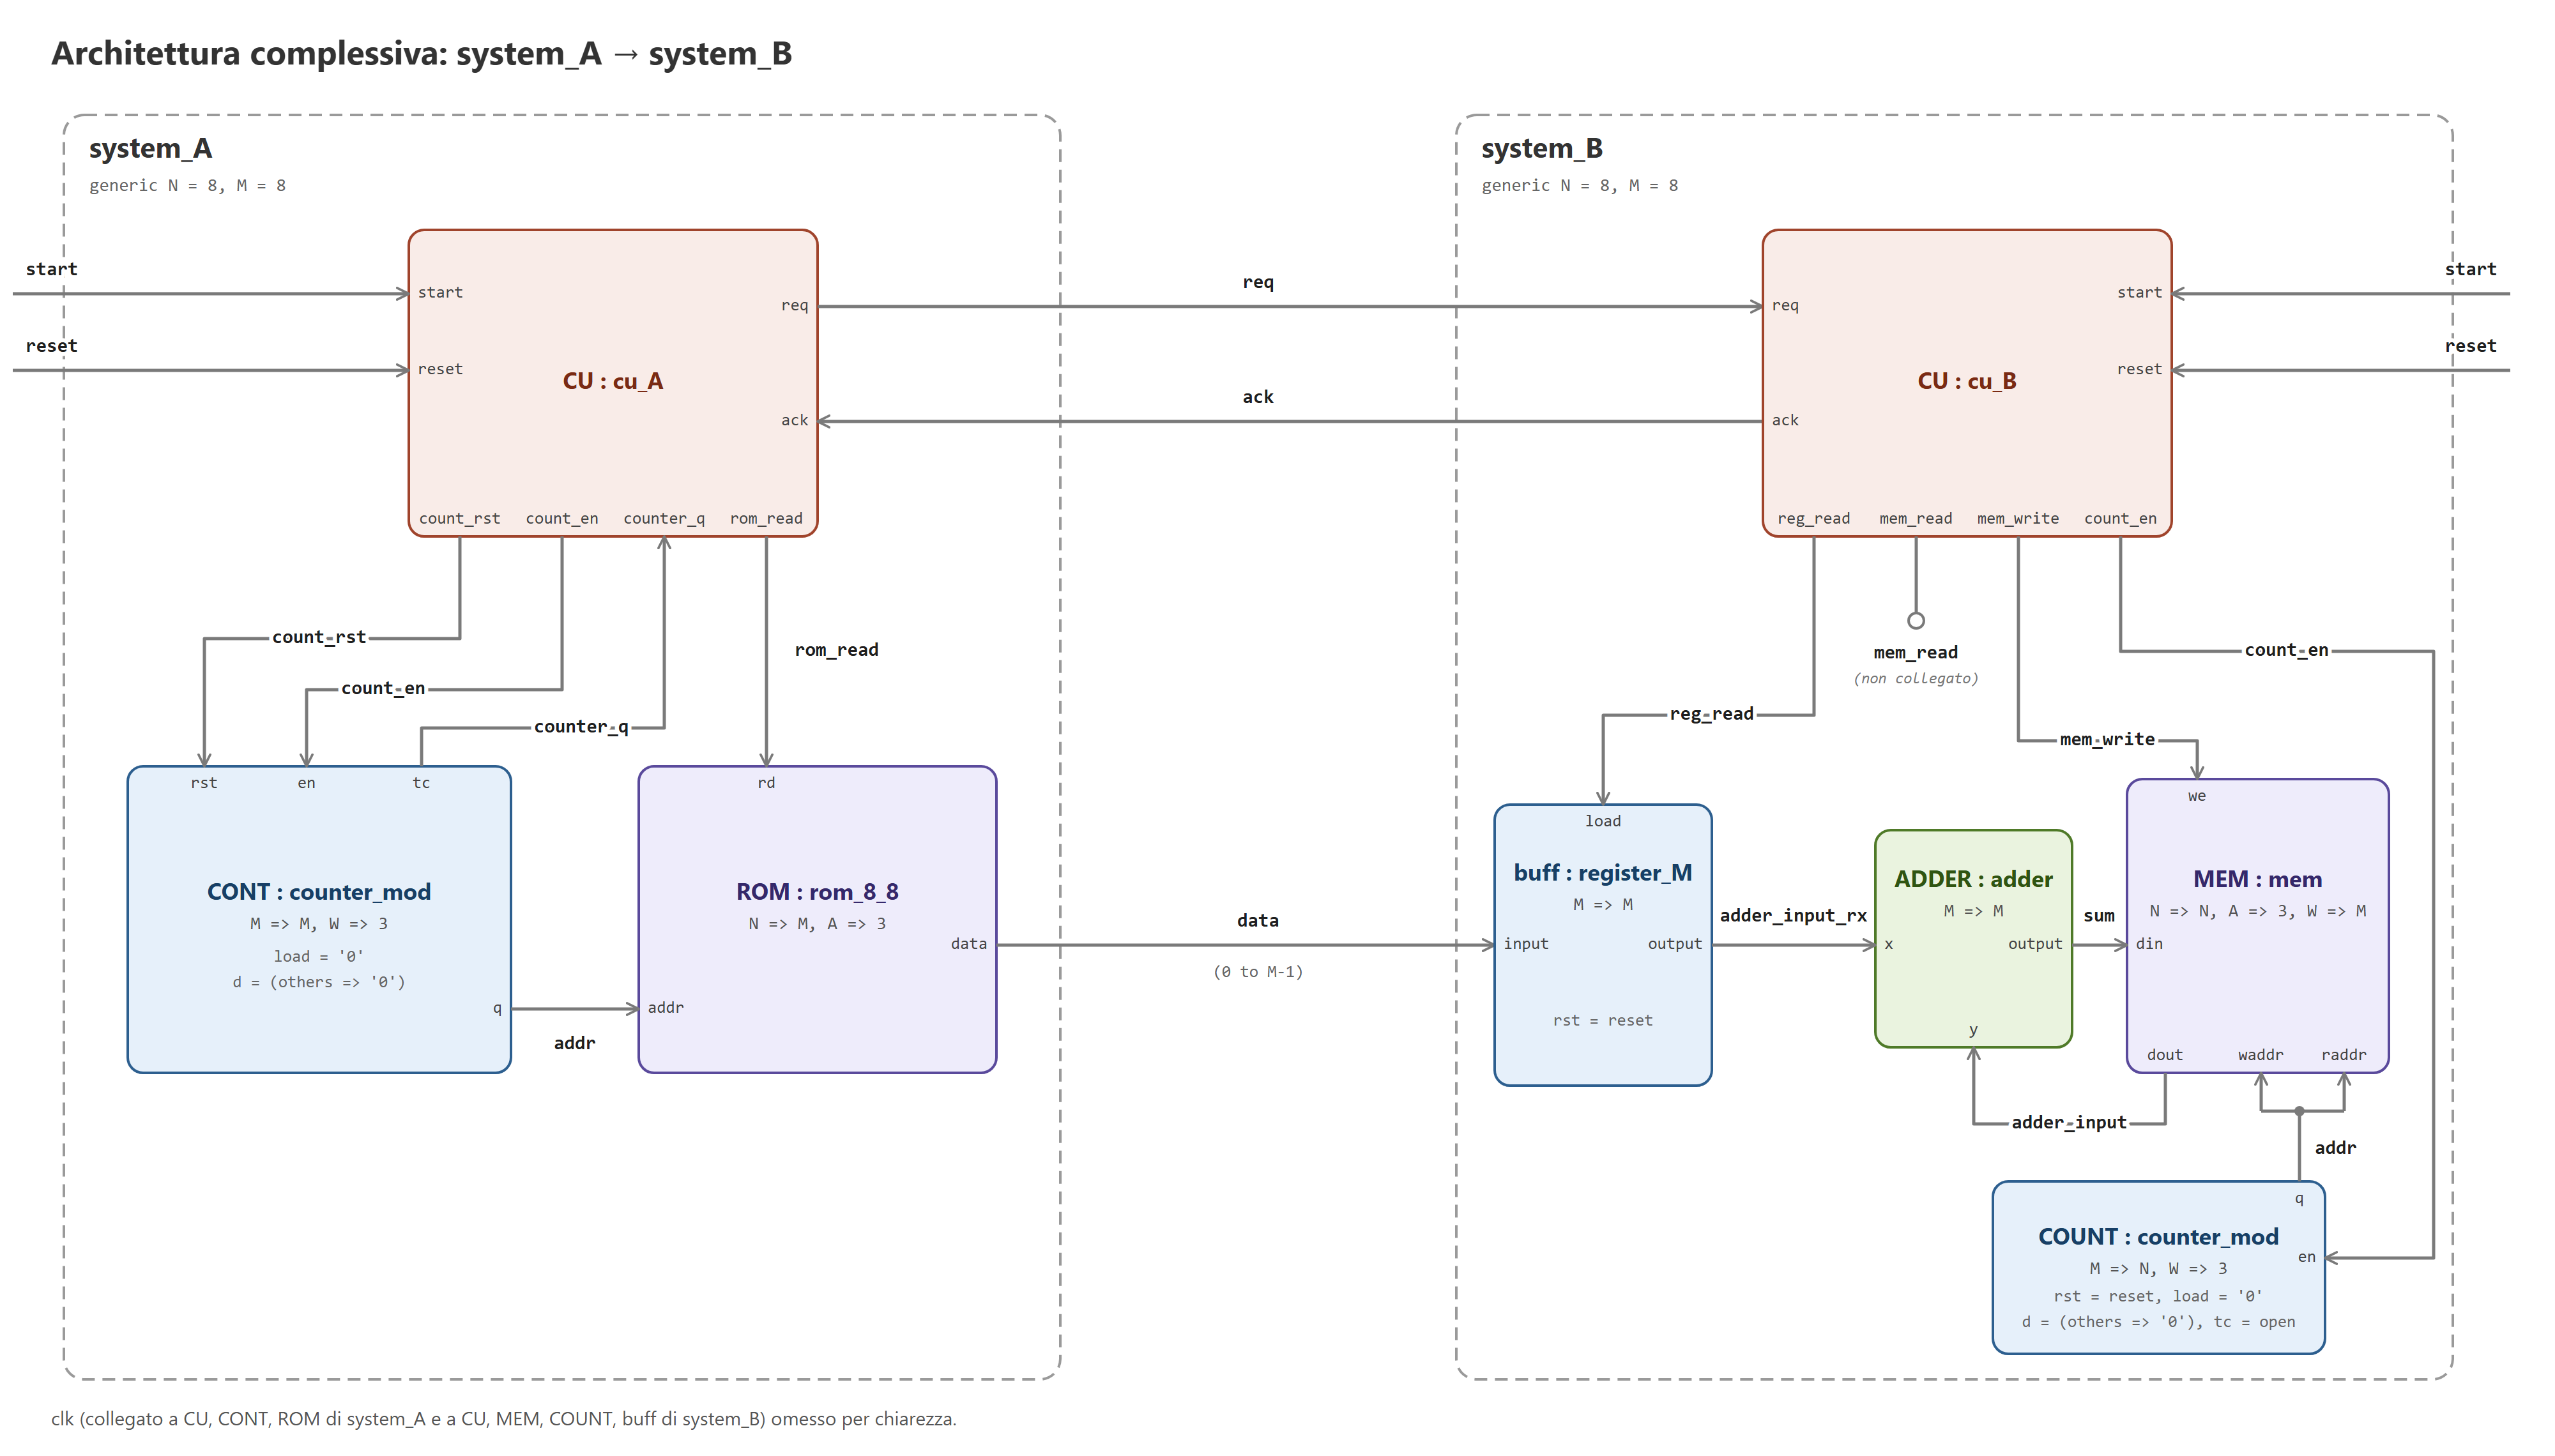
\includegraphics[width=\linewidth]{figure/esercizio8-1/architettura}
  \caption{Architettura del sistema di handshaking}
  \label{fig:esercizio8-1:architettura}
\end{figure}

Il protocollo è a quattro fasi. A porta \texttt{req} a \texttt{'1'} dopo aver letto il dato dalla ROM e attende \texttt{ack} a \texttt{'1'}; B, visto \texttt{req}, cattura il dato nel registro e alza \texttt{ack}; A abbassa \texttt{req}; B, rilevato \texttt{req} a \texttt{'0'}, scrive la somma in memoria, incrementa il contatore e abbassa \texttt{ack}. Solo a questo punto A passa alla stringa successiva. Le unità di controllo sono descritte dalle FSM nelle figure~\ref{fig:esercizio8-1:fsm-a} e~\ref{fig:esercizio8-1:fsm-b}.

\begin{figure}[H]
  \centering
  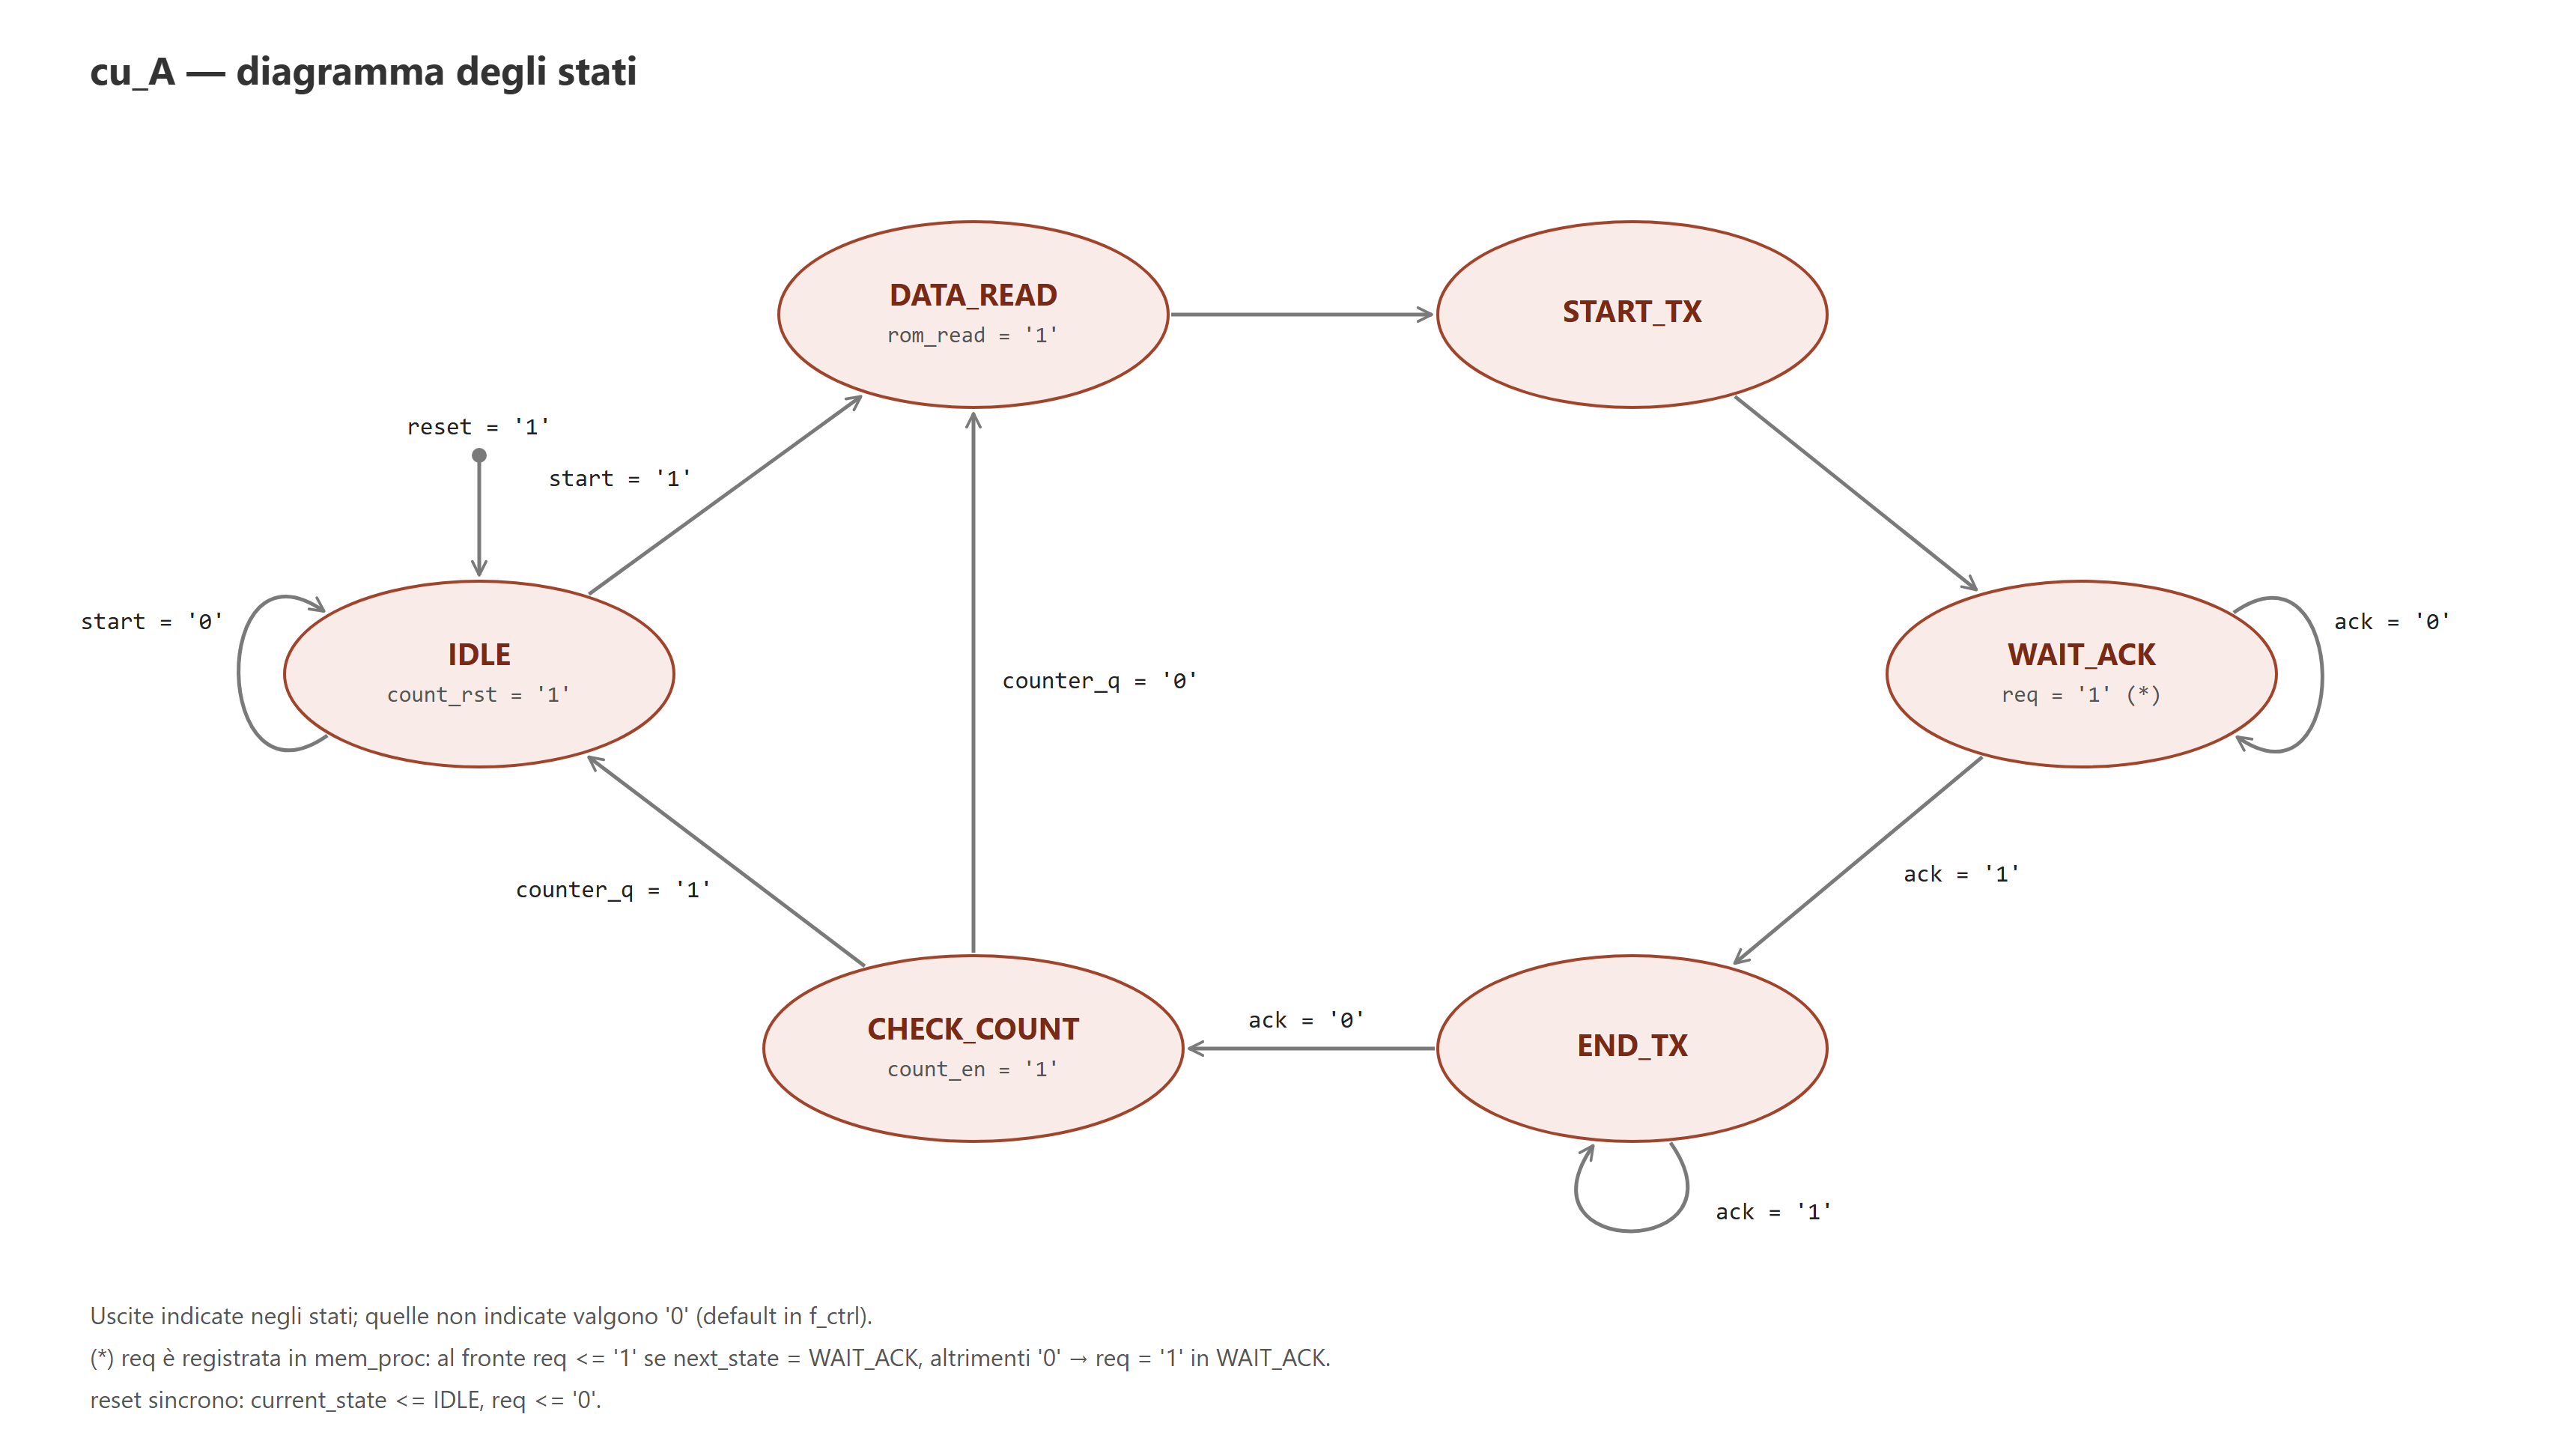
\includegraphics[width=0.8\linewidth]{figure/esercizio8-1/fsm-a}
  \caption{FSM dell'unità A}
  \label{fig:esercizio8-1:fsm-a}
\end{figure}

\begin{figure}[H]
  \centering
  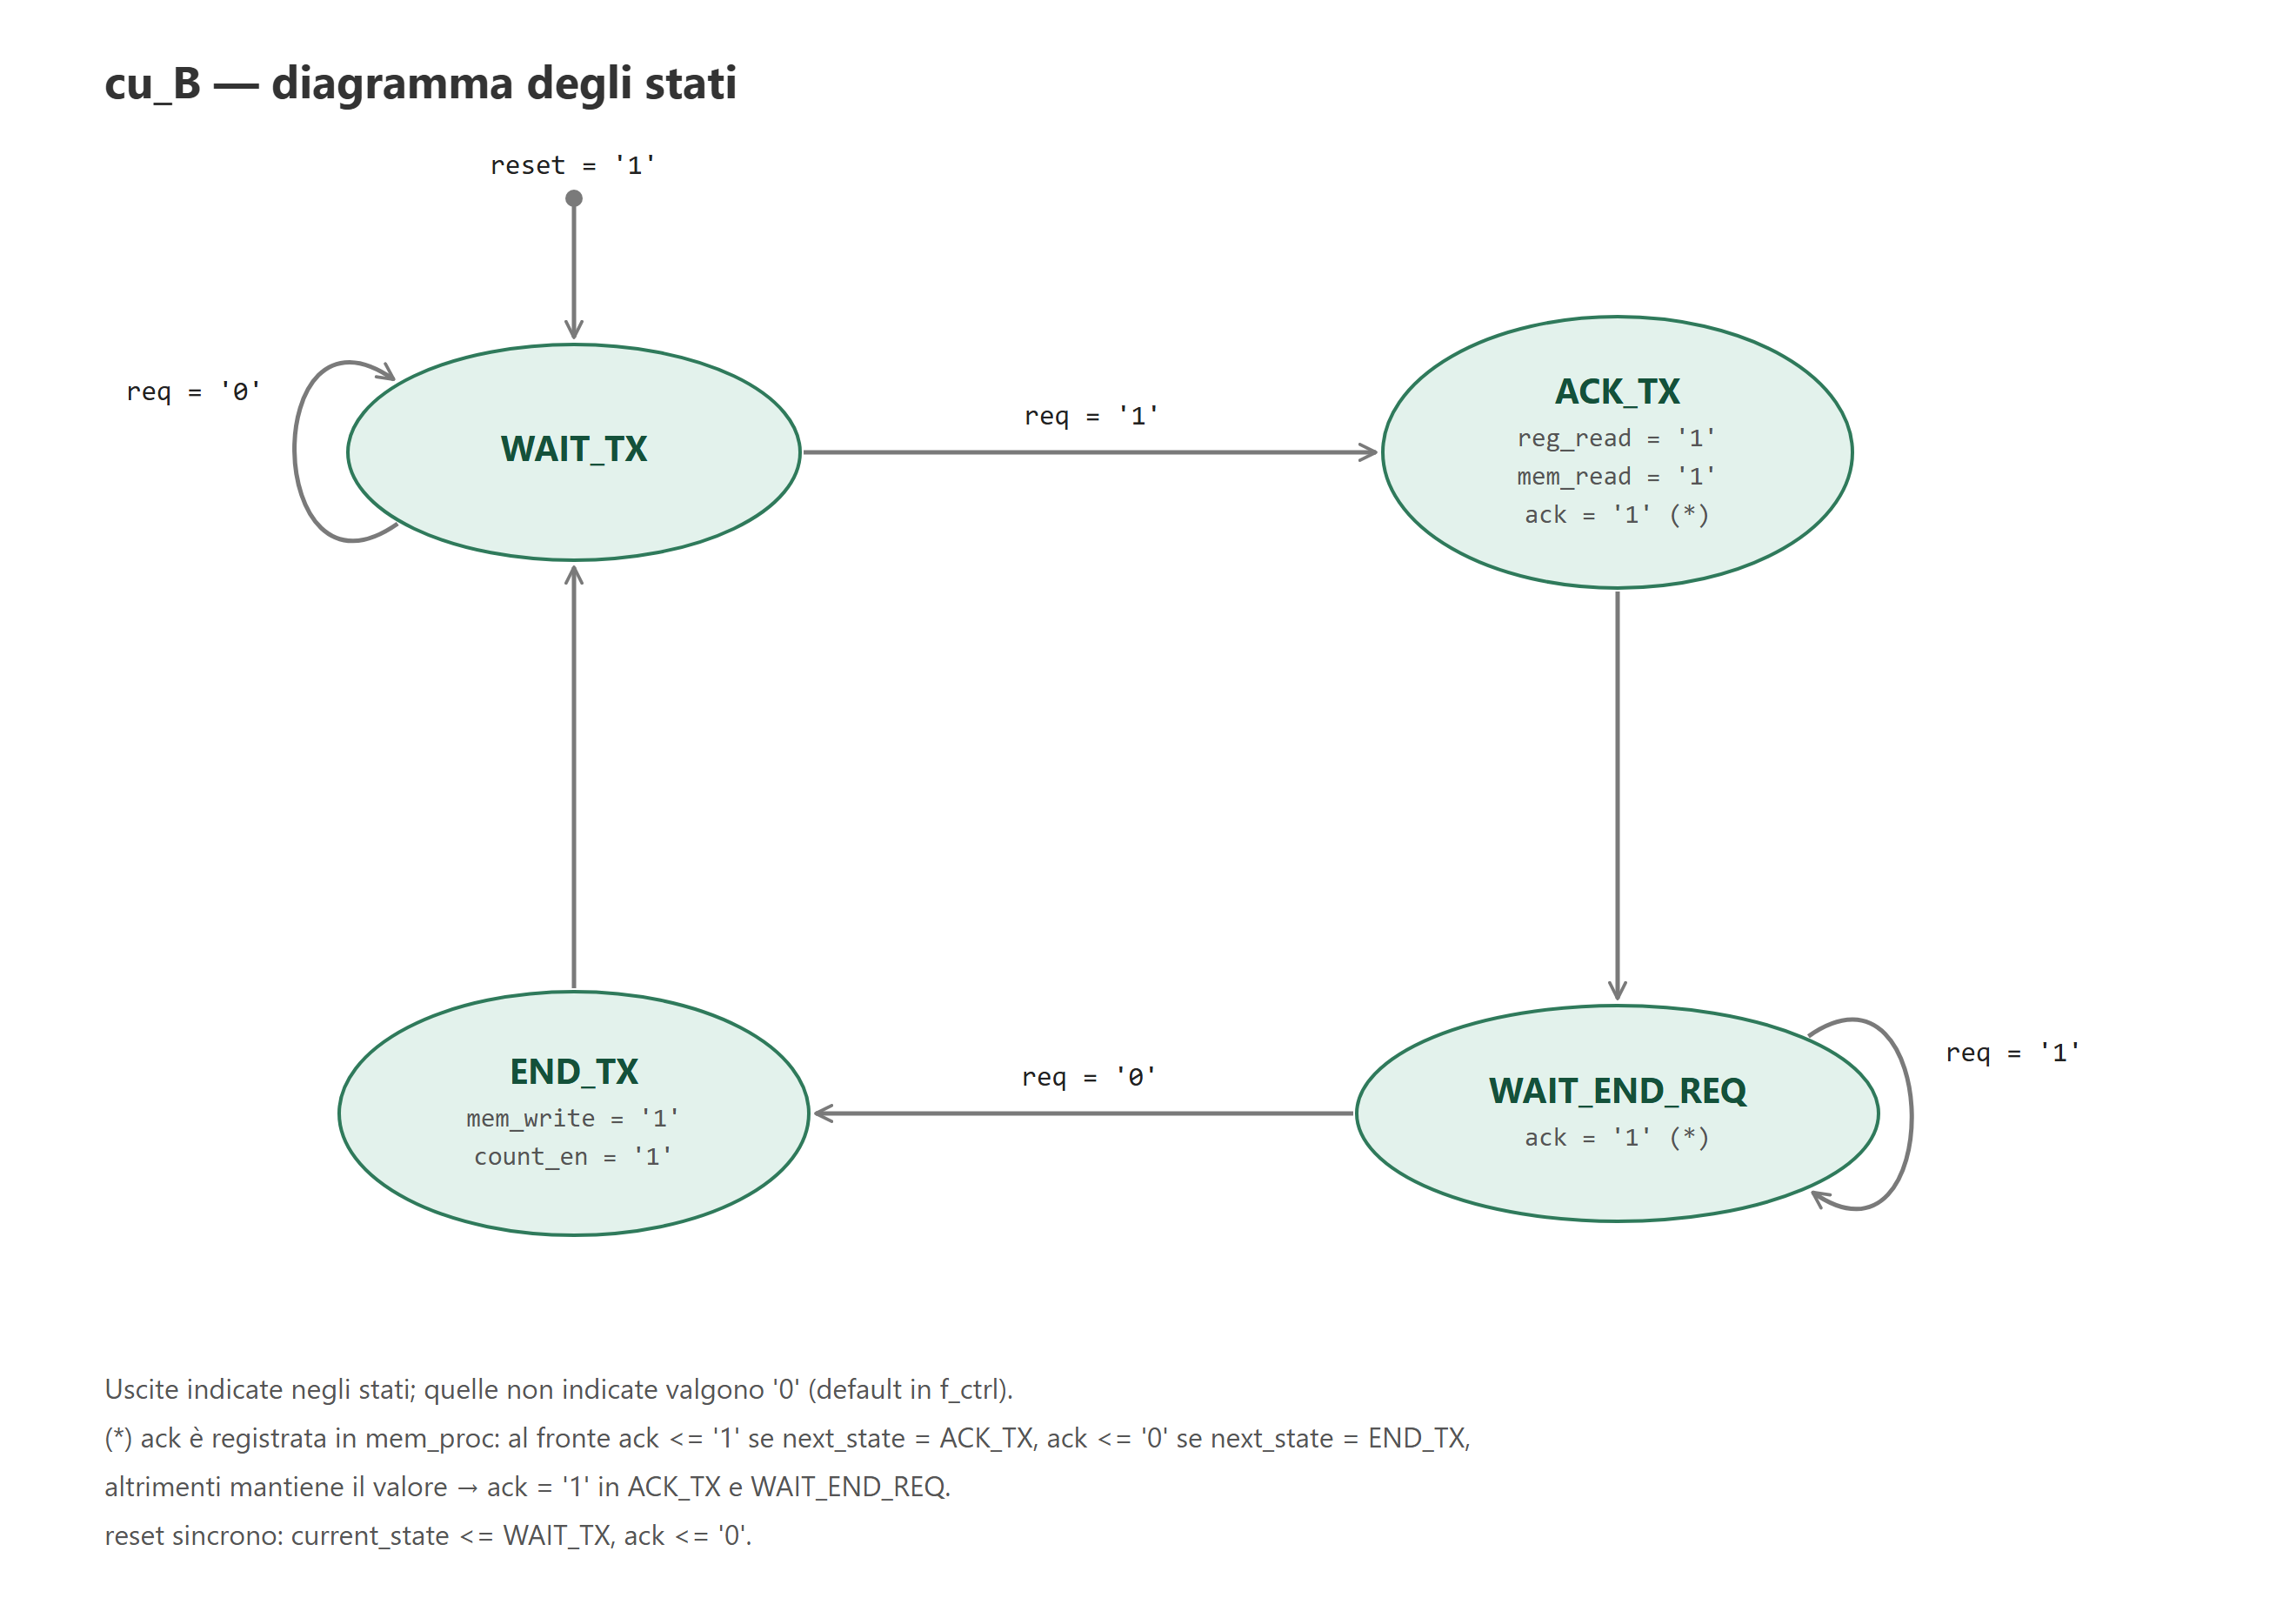
\includegraphics[width=0.6\linewidth]{figure/esercizio8-1/fsm-b}
  \caption{FSM dell'unità B}
  \label{fig:esercizio8-1:fsm-b}
\end{figure}

Nelle figure le uscite non indicate in uno stato valgono \texttt{'0'}; \texttt{req} e \texttt{ack} sono uscite registrate, aggiornate al fronte di clock in funzione dello stato successivo (segnalate con un asterisco). L'FSM di A ha sei stati (\texttt{IDLE}, \texttt{DATA\_READ}, \texttt{START\_TX}, \texttt{WAIT\_ACK}, \texttt{END\_TX}, \texttt{CHECK\_COUNT}) e quella di B quattro (\texttt{WAIT\_TX}, \texttt{ACK\_TX}, \texttt{WAIT\_END\_REQ}, \texttt{END\_TX}).

\begin{osservazione}
Rispetto alla soluzione proposta, l'implementazione differisce nei seguenti punti:
\begin{itemize}
  \item le unità di controllo sono \texttt{cu\_A} e \texttt{cu\_B}, con porte \texttt{clk}, \texttt{count\_en} e \texttt{count\_rst} (invece di \texttt{clock}, \texttt{counter\_enable} e \texttt{counter\_reset});
  \item la FSM di A include \texttt{WAIT\_ACK} (non \texttt{DATA\_WAIT}) e non usa one-hot esplicita;
  \item le FSM sono descritte con due process distinti (combinatorio e sequenziale);
  \item la ROM del nodo A è \texttt{rom\_8\_8} con contenuto fisso;
  \item memoria e contatore sono componenti comuni;
  \item \texttt{cu\_B} riceve \texttt{start} inutilizzato e l'uscita \texttt{mem\_read} non è collegata.
\end{itemize}
\end{osservazione}

\implementazione

Il contatore \texttt{counter\_mod} (listato~\ref{lst:esercizio5-1:counter-mod}) e la memoria \texttt{mem} (listato~\ref{lst:esercizio6-1:mem}) sono già stati presentati e vengono istanziati senza modifiche. Il componente \texttt{rom} (listato~\ref{lst:esercizio6-1:rom}), pur incluso nel progetto Vivado, non è istanziato in questo esercizio: il nodo A usa la ROM dedicata \texttt{rom\_8\_8}. Vediamo ora i componenti propri dell'esercizio, partendo dal nodo B.

Il registro \texttt{register\_M} ha larghezza $M$ (generic, default 8) e porte \texttt{clk}, \texttt{rst}, \texttt{load}, \texttt{input} e \texttt{output}. Un process sincrono azzera il dato con \texttt{rst} attivo e lo carica al fronte di salita quando \texttt{load} è \texttt{'1'}.

\vhdlfile{esercizio8-1/register_m.vhd}{Implementazione del registro}{lst:esercizio8-1:register-m}

L'\texttt{adder} ha architettura dataflow e somma i due ingressi \texttt{x} e \texttt{y} di $M$ bit, interpretati come \texttt{unsigned}. L'uscita \texttt{output} ha gli stessi $M$ bit, quindi il riporto viene scartato.

\vhdlfile{esercizio8-1/adder.vhd}{Implementazione dell'adder}{lst:esercizio8-1:adder}

La \texttt{rom\_8\_8} ha generic \texttt{N} (locazioni) e \texttt{A} (bit di indirizzo) e memorizza in una costante otto byte: \texttt{x"00"}, \texttt{x"FF"}, \texttt{x"01"}, \texttt{x"80"}, \texttt{x"0F"}, \texttt{x"F0"}, \texttt{x"AA"}, \texttt{x"55"}. Un'\texttt{assert} verifica che \texttt{N} sia indirizzabile su \texttt{A} bit; la lettura è sincrona, controllata da \texttt{rd}.

\vhdlfile{esercizio8-1/rom_8_8.vhd}{Implementazione della ROM 8x8}{lst:esercizio8-1:rom-8-8}

L'unità di controllo \texttt{cu\_A} è descritta con due process. Il process \texttt{f\_ctrl}, combinatorio, calcola stato successivo e uscite (\texttt{count\_rst} in \texttt{IDLE}, \texttt{rom\_read} in \texttt{DATA\_READ}, \texttt{count\_en} in \texttt{CHECK\_COUNT}); il process \texttt{mem\_proc}, sincrono, aggiorna lo stato e registra \texttt{req}, che vale \texttt{'1'} quando lo stato successivo è \texttt{WAIT\_ACK}. In \texttt{CHECK\_COUNT} l'ingresso \texttt{counter\_q} decide se tornare a \texttt{IDLE} (ultima stringa) o proseguire con \texttt{DATA\_READ}.

\vhdlfile{esercizio8-1/cu_a.vhd}{Implementazione della CU A}{lst:esercizio8-1:cu-a}

L'unità \texttt{cu\_B} ha la stessa struttura a due process: in \texttt{ACK\_TX} attiva \texttt{reg\_read} e \texttt{mem\_read}; in \texttt{END\_TX} attiva \texttt{mem\_write} e \texttt{count\_en}. L'uscita \texttt{ack}, registrata, sale quando lo stato successivo è \texttt{ACK\_TX}, scende quando è \texttt{END\_TX} e negli altri casi mantiene il valore.

\vhdlfile{esercizio8-1/cu_b.vhd}{Implementazione della CU B}{lst:esercizio8-1:cu-b}

Il top module del nodo A, \texttt{system\_A}, ha generic \texttt{N} e \texttt{M} e istanzia tramite port mapping la \texttt{cu\_A}, un \texttt{counter\_mod} (con \texttt{W} pari a 3, reset da \texttt{count\_rst}, abilitazione da \texttt{count\_en} e riporto \texttt{tc} verso \texttt{counter\_q}) e la \texttt{rom\_8\_8}, indirizzata dall'uscita del contatore.

\vhdlfile{esercizio8-1/system_a.vhd}{Implementazione del sistema A}{lst:esercizio8-1:system-a}

Il top module del nodo B, \texttt{system\_B}, istanzia \texttt{cu\_B}, \texttt{mem}, un \texttt{counter\_mod}, l'\texttt{adder} e il registro \texttt{buff}. Il registro cattura il dato ricevuto quando \texttt{reg\_read} è alto; l'adder somma il contenuto del registro (\texttt{adder\_input\_rx}) al valore letto dalla memoria all'indirizzo corrente (\texttt{adder\_input}); il risultato \texttt{sum} viene scritto nella stessa locazione quando \texttt{mem\_write} è alto. Lo stesso indirizzo pilota lettura e scrittura, e l'uscita di terminal count del contatore non è utilizzata.

\vhdlfile{esercizio8-1/system_b.vhd}{Implementazione del sistema B}{lst:esercizio8-1:system-b}

\simulazione

Il testbench \texttt{handshaking\_tb} ha entità senza porte e istanzia \texttt{system\_A} (\texttt{sysA}) e \texttt{system\_B} (\texttt{sysB}) con $N = M = 8$, collegando \texttt{req}, \texttt{ack} e \texttt{data}. Due process, \texttt{clockA} e \texttt{clockB}, generano clock con periodo di \SI{10}{ns} e \SI{11}{ns}, per verificare il funzionamento con clock diversi. Il process \texttt{stim\_proc} attende \SI{100}{ns}, impone \texttt{rst} per \SI{10}{ns}, attende altri \SI{10}{ns}, alza \texttt{start} per \SI{10}{ns} e termina con \texttt{wait;}. Non sono presenti \texttt{assert}: il controllo avviene per ispezione delle forme d'onda.

\vhdlfile{esercizio8-1/handshaking_tb.vhd}{Testbench dell'handshaking}{lst:esercizio8-1:handshaking-tb}

Il risultato della simulazione è riportato in figura~\ref{fig:esercizio8-1:simulazione}. Il segnale \texttt{data} e la ROM sono mostrati in decimale con segno.

\begin{figure}[H]
  \centering
  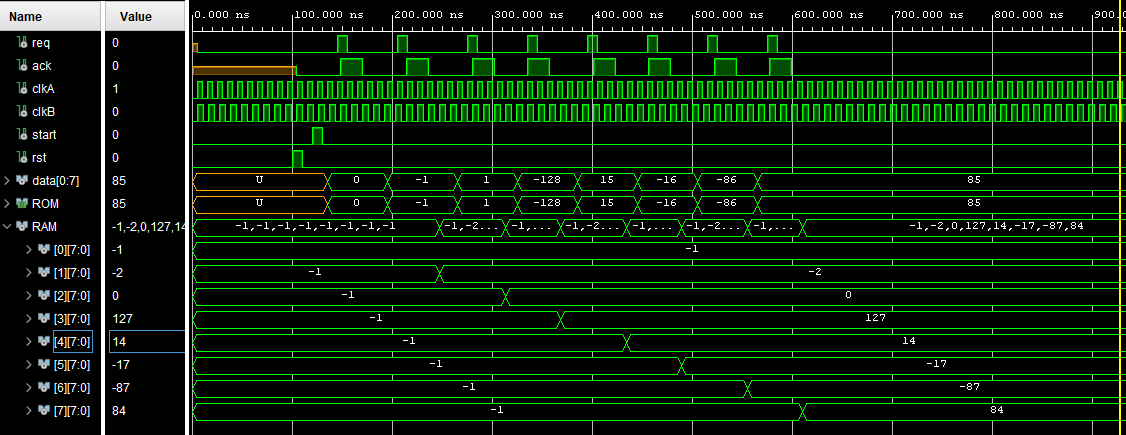
\includegraphics[width=\linewidth]{figure/esercizio8-1/simulazione}
  \caption{Simulazione dell'handshaking}
  \label{fig:esercizio8-1:simulazione}
\end{figure}

Dopo \texttt{start} si osservano otto impulsi di \texttt{req}, ciascuno seguito da un impulso di \texttt{ack} (di durata maggiore, perché \texttt{ack} scende solo dopo che B ha visto \texttt{req} a \texttt{'0'}). Su \texttt{data} compaiono in sequenza i valori della ROM: $0$, $-1$, $1$, $-128$, $15$, $-16$, $-86$, $85$, ossia \texttt{x"00"}, \texttt{x"FF"}, \texttt{x"01"}, \texttt{x"80"}, \texttt{x"0F"}, \texttt{x"F0"}, \texttt{x"AA"}, \texttt{x"55"}. La memoria \texttt{RAM} del nodo B ha inizialmente valore $-1$ (\texttt{x"FF"}) in ogni locazione e viene aggiornata una locazione per volta al termine di ciascun trasferimento. Ad esempio, per la locazione 3 il dato ricevuto è \texttt{x"80"} ($-128$): la somma $\texttt{x"80"} + \texttt{x"FF"}$ dà \texttt{x"7F"} sugli 8 bit, cioè $127$, valore effettivamente letto in \texttt{RAM[3]}. Al termine il contenuto è $-1, -2, 0, 127, 14, -17, -87, 84$.

\begin{risultato}
Le otto somme sono memorizzate nella memoria di B come mostrato in figura, con i due nodi su clock a \SI{10}{ns} e \SI{11}{ns}.
\end{risultato}
